Scientists from the worlds of applied math and neurology have only recently started investigating the relationships between chimera states and epileptic seizures \autocite{Santos2017,Andrzejak2016,Wang2012}.
While the ideas of using computer modeling for seizures have been around for over a decade \autocite{Lytton2008}, the power and speed of those models has drastically increased, and allowed us to investigate ever more complicated situations.
Many models for the brain, including all of those discussed in this proposal, view the brain as a network of coupled oscillators.

One way to investigate the dynamics of an epileptic seizure is through what is known as a lumped model \autocite{Baier2012}.
This technique allows researchers to model large clusters of neurons and regions as a single lump that acts together.
For example, a lumped model could describe seizures as one excitatory process and two inhibitory processes brain-wide, operating on different time scales.
In such a model, we see a recreation of the four archetypal seizure patterns, as well as transitions between them, which are observed in measured data \autocite{Wang2012}.

One of the benefits of lumped modeling is that it generally results in fairly simple models.
Being able to accurately describe some of the behavior of the entire human brain using only three coupled differential equations provides a relatively easy system to comprehend.
However, using this high of a level of abstraction does have its downsides.
In order to condense the behavior of a complex system like the brain to such a simple model means necessary loss of information \autocite{Lytton2008}.
As an example, we will use the model mentioned before, which lumps the brain into one excitatory and two inhibitory processes.
This model is described by the following set of equations:
\begin{align}
  \label{eq:x}
  \tau_{x}
  \dv{x}{t}
  &=
    -x
    +
    S(C_{x, x} x + C_{x, y} y + C_{x, z} z + P) \\
  \label{eq:y}
  \tau_{y}
  \dv{y}{t}
  &=
    -y
    +
    S(C_{y, x} x + C_{y, y} y + C_{y, z} z + Q) \\
  \label{eq:z}
  \tau_{z}
  \dv{z}{t}
  &=
    -z
    +
    S(C_{z, x} x + C_{z, y} y + C_{z, z} z + R)
\end{align}
where $x$ represents the excitatory process, $y$ represents a fast inhibitory process, $z$ represents a slow inhibitory process \autocite{Wang2012}.
The function $S$ represents an activation function, the parameters $C_{i, j}$ represent the strength of the relationship between process $i$ and process $j$, and $\tau_{i}$ represents the time scale of process $i$ (fast in the case of $x$ and $y$, slow in the case of $z$).
Finally, the parameters $P$, $Q$, and $R$ represent external inputs or excitability of the processes.

This can be a relatively easy system to solve and understand, depending on the choice of $S$.
However, that comes at a cost.
Describing the entire function of the brain as three equations results in an aphysical model.
While the coupled oscillators described in \cref{eq:x,eq:y,eq:z} are relatively simple and show complex behavior, they are not all that helpful as diagnostic or prediction tools.
This is because the brain is made of many more than three interacting components.
A helpful analogy is as follows.
Each of the pixels on a television or computer screen is made up of three lights: one red, one blue, one green.
The colors that we see are actually combinations of these red, green, and blue lights, so close together that we can see them as white, or yellow, or puce.
In order to fully describe the screen of my computer, which has a resolution of 2560 $\times$ 1600 pixels, we would need 2560 $\times$ 1600 $\times$ 3 = 12288000 different numbers.
If you pulled up a picture of a puppy (\cref{fig:puppy}) and asked me to describe it, you would not be satisfied with my telling you ``Well, your screen is, on average, using its red at \SI{51}{\percent}, its blue at \SI{54}{\percent}, and its green at \SI{34}{\percent}.''
All you would be able to gain from that is that your screen is, on average, brown-ish green (\cref{fig:bland}).
This does tell you something (the picture is probably not of a whale), but not as much information as you likely wanted.
If you wanted to crop out the grass on the right side of the figure, you would not be able to do so with the little information I had given you.
Similarly, using a lumped model can give us information about overall brain activity, but can not give us enough to figure out where specifically problems are, and where they are coming from.
Thus, we need to turn to other modeling techniques.

\begin{figure}[ht]
  \centering
  \begin{subfigure}[c]{0.4\textwidth}
    \includegraphics[width=\textwidth]{figure/lumped}
    \caption{}
    \label{fig:lumped}
  \end{subfigure} $\iff$
  \begin{subfigure}[c]{0.4\textwidth}
    
\includegraphics[width=\textwidth]{figure/bland}
    \caption{}
    \label{fig:bland}
  \end{subfigure}

  \begin{subfigure}[c]{0.4\textwidth}
    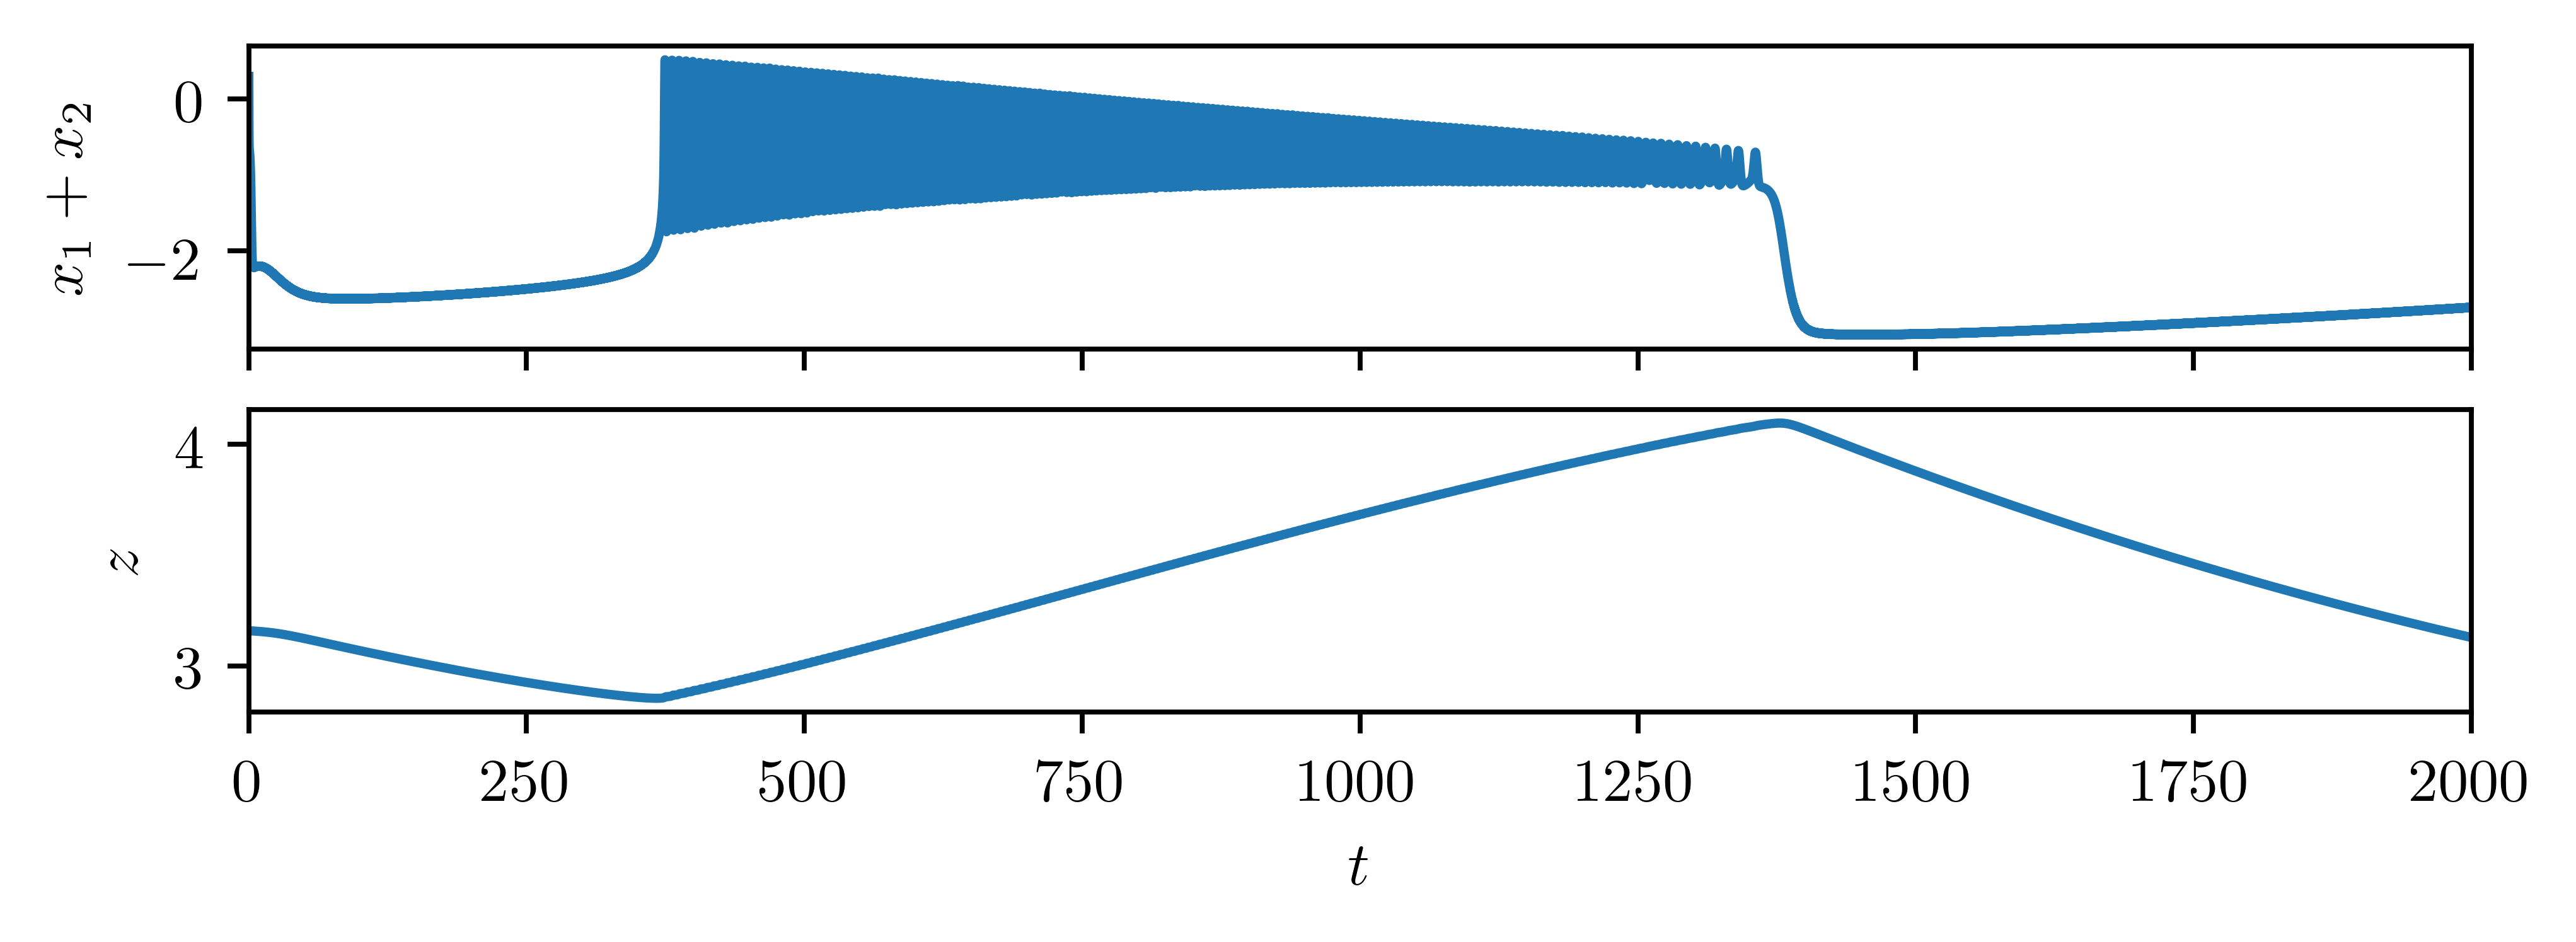
\includegraphics[width=\textwidth]{figure/epileptor}
    \caption{}
    \label{fig:epileptor}
  \end{subfigure} $\iff$
  \begin{subfigure}[c]{0.4\textwidth}
    
\includegraphics[width=\textwidth]{figure/midres}
    \caption{}
    \label{fig:midres}
  \end{subfigure}

  \begin{subfigure}[c]{0.4\textwidth}
    
\includegraphics[width=\textwidth]{figure/HR}
    \caption{}
    \label{fig:HR}
  \end{subfigure} $\iff$
  \begin{subfigure}[c]{0.4\textwidth}
    
\includegraphics[width=\textwidth]{figure/puppy}
    \caption{}
    \label{fig:puppy}
  \end{subfigure}
  \caption{\Cref{fig:lumped} shows the model of Wang \etal, which gives a broad overview of brain activity.
  It reduces the extremely complex system of the brain to three dimensions, making it a relatively simple mathematical problem.
  However, much like describing the picture of the puppy as three RGB values (\cref{fig:bland}) sacrifices all spatial information and nuance from the photograph, using just three equations to describe the entire brain deprives us of a lot of knowledge of what is going on inside the various parts of the brain.
  \Cref{fig:epileptor} shows the Epileptor model, which describes the state of the brain as a whole.
  It takes into account the physical states of neurons around the brain, but still uses some simplifications that make it difficult to get an accurate picture of the state of the brain.
  This is like describing the puppy by giving information about a few key pixels, while still leaving a lot of information out.
  Finally, \cref{fig:HR} shows the HR model, which can be used at varying levels of precision.
  If we had perfect information about the connective structure of the brain, we could recreate its interactions perfectly using the HR model (\cref{fig:puppy}).
}
  \label{fig:analogy}
\end{figure}

The key alternative modeling technique is that of using a neuronal network \autocite{Lytton2008}.
This involves directly modeling networks of neurons.
As with any model, it comes with its benefits and downsides.
The two main downsides are first that an overly detailed model can negate the benefits that come from using an abstracting model in the first place, and the fact that detailed models require more computing power \autocite{Lytton2008}.
However, computing power improves exponentially with time, making larger-scale and more detailed models more useful as time goes on.

The benefits derived from these detailed models are noteworthy, as well.
As an example, a neuronal network model could describe the interactions between 65 different cortical areas via 1139 connections \autocite{Santos2017}.
The behavior of each area is described by the Hindmarsh-Rose (HR) neuron model, which is characterized by a set of coupled nonlinear differential equations.
These equations are not solvable analytically, but can be investigated numerically.
Additionally, each aspect of the equations corresponds to a measurable physical quantity.
Returning to the puppy analogy, these models give a wealth of information; instead of giving you a list of three numbers to describe the color of the whole picture, I could give you the RGB values for each pixel.
This would be overwhelming for you to deal with by yourself, but easy for a computer to convert into a perfectly clear picture of a puppy.
Similarly, the model is relatively easy to manage with sufficient computing power.

This specific model has exhibited some very interesting properties.
Chiefly, it has shown a propensity for chimera states, which are a deeply studied area in the world of nonlinear dynamics \autocite{Santos2017,Martens2013}.
Since chimera states have been observed for specific parameter values in this type of network, it would provide a good testing ground for analogies between epileptic seizures and collapses of chimera states into fully synchronous regimes \autocite{Andrzejak2016}.
The behavior of any model is supposed to directly mimic the behavior of the system it is modeling.
If the model exhibits a chimera state for a certain set of parameter values, then the brain should be in a chimera state for those same parameter values.
When the model shows a whole cortex of oscillating synchronously, while the rest of the brain oscillates asynchronously, the model is describing a focal seizure.
When this chimera state collapses into total synchrony, the model is describing secondary generalization of the seizure.
As the parameters of the model change over time (due to various chemical and environmental factors in the brain), the likelihood of chimera states (and therefore seizures) also changes.
However, given the recency of the publications making these claims, the comparisons have not been tested, and therefore provide a set of open questions for further exploration.

A model of an intermediate level of abstraction is commonly referred to as Epileptor \autocite{Jirsa2014}.
It lumps the brain into inhibitory and excitatory processes, operating at different time scales, but describes some of the behavior of these lumps using a physically-grounded model.
This model allows researchers to understand the system's behavior quite well, and use standard techniques of nonlinear dynamics in order to study its properties.
Its predictions match with data very well, but has some parameters which are not directly measurable, i.e., do not have a direct correspondence with a physiological state of a part of the brain.
This immeasurability makes Epileptor difficult to use as a real-time predictor of seizures, but does provide some insight into the mechanisms behind them.
For example, Epileptor's predictions include the phenomenon known as critical slowing-down \autocite{Jirsa2014}.
This means that, as a seizure approaches, any changes from the brain's normal baseline activity take much longer to return to normal.
This is a commonly observed phenomenon in many nonlinear systems, and Epileptor's predictions of its presence match with what has been observed \autocite{Scheffer2009}.

%%% Local Variables:
%%% mode: latex
%%% TeX-engine: xetex
%%% TeX-master: "../main"
%%% End:
